\subsection{Integration of a vector-valued function with respect to a vectorial measure}

PROPOSITION 11. --- Let F, G, H be three Banach spaces, \(\Phi\) a continuous bilinear mapping of F × G into H. Let m be a majorizable vectorial measure on T, with values in G. Then there exists one and only one continuous linear mapping I \(_{\Phi,\mathbf{m}}\) of \(\overline{\mathcal{L}}_{\mathrm{F}}^{1}(|\mathbf{m}|)\) into H such that, for every z ∈ F and every numerical function h integrable for \textbar m\textbar, one has I \(_{\Phi,\mathbf{m}}(hz) = \Phi(z, \int h dm)\) . Moreover,

\[
\left| \mathrm{I} _ {\Phi , \mathbf {m}} (\mathbf {f}) \right| \leqslant \| \Phi \| \int | \mathbf {f} | d | \mathbf {m} |\tag{4}
\]

for every function \(\mathbf{f} \in \overline{\mathcal{L}}_{\mathrm{F}}^{1}(|\mathbf{m}|)\) .

If there exists such a mapping, its value for a step function \(\mathbf{f}\) over the \(|\mathbf{m}|\) -integrable sets is uniquely determined: for, it is known that one can then write \(\mathbf{f} = \sum_{i} \mathbf{a}_{i} \varphi_{\mathrm{X}_{i}}\) , where the \(\mathrm{X}_{i}\) are \(|\mathbf{m}|\) -integrable and disjoint, and the \(\mathbf{a}_{i} \in \mathrm{F}\) (Ch. IV, §4, No.~9, Lemma). The value of \(\mathrm{I}_{\Phi, \mathbf{m}}(\mathbf{f})\) must therefore be equal to \(\sum_{i} \Phi(\mathbf{a}_{i}, \int \varphi_{\mathrm{X}_{i}} d\mathbf{m})\) . Now, we have (No.~3, Prop. 5)

\[
\left| \sum_ {i} \Phi (\mathbf {a} _ {i}, \int \varphi_ {\mathrm{X} _ {i}} d \mathbf {m}) \right| \leqslant \| \Phi \| \cdot \sum_ {i} | \mathbf {a} _ {i} | \cdot | \mathbf {m} | (\mathrm{X} _ {i}) = \| \Phi \| \int | \mathbf {f} | d | \mathbf {m} |,\tag{5}
\]

which shows first of all that the element \(\sum_{i} \Phi(a_i, \int \varphi_{X_i} d\mathbf{m})\) of H does not depend on the particular expression of \(\mathbf{f}\) in the form \(\sum_{i} a_i \varphi_{X_i}\) , hence that we may denote it by \(I_{\Phi, \mathbf{m}}(\mathbf{f})\) . One verifies immediately that the mapping \(I_{\Phi, \mathbf{m}}\) so defined is linear on the space \(\mathcal{E}_F\) of step functions over the \(|\mathbf{m}|\) -integrable sets: for, it suffices to write two functions \(\mathbf{f}, \mathbf{g}\) of \(\mathcal{E}_F\) in the form \(\mathbf{f} = \sum_{i} a_i \varphi_{X_i}\) and \(\mathbf{g} = \sum_{i} b_i \varphi_{X_i}\) with the same finite family of pairwise disjoint \(|\mathbf{m}|\) -integrable sets \(X_i\) (which is possible by virtue of the Lemma of Ch. IV, §4, No.~9). The inequality (5) then shows that \(I_{\Phi, \mathbf{m}}\) is continuous on \(\mathcal{E}_F\) , and since this subspace is dense in \(\overline{\mathscr{L}}_F^1\) (Ch. IV, §4, No.~10, Cor. 1 of Prop. 19 and Ch. V, §1, No.~3), one deduces from this the existence and uniqueness of \(I_{\Phi,m}\) , as well as the inequality (4).

One says that \(I_{\Phi,\mathbf{m}}(\mathbf{f})\) is the integral of f with respect to m (relative to the bilinear mapping \(\Phi\) ); when the value of the bilinear mapping \(\Phi\) at the point \((\mathbf{x},\mathbf{y})\) is denoted xy, we shall write \(\int f dm\) instead of \(I_{\Phi,\mathbf{m}}(\mathbf{f})\) .

With the notations of No.~6, the integral \(\int \langle \mathbf{f},\mathbf{g}\rangle d\mu\) is none other than \(\mathrm{I}_{\Phi ,\mathbf{m}}(\mathbf{f})\) with \(\Phi (\mathbf{x},\mathbf{x}^{\prime}) = \langle \mathbf{x},\mathbf{x}^{\prime}\rangle\) and \(\mathbf{m} = \mathbf{g}\cdot \mu\)

COROLLARY. --- If m and \(m'\) are two majorizable measures on T, with values in G, then \(I_{\Phi,m+m'} = I_{\Phi,m} + I_{\Phi,m'}\) and \(I_{\Phi,\lambda m} = \lambda I_{\Phi,m}\) for every scalar \(\lambda\) .

The second assertion is immediate. The first signifies that for every function f that is both \(|m|\) -integrable and \(|m'|\) -integrable,

\[
\mathrm{I} _ {\Phi , \mathbf {m} + \mathbf {m} ^ {\prime}} (\mathbf {f}) = \mathrm{I} _ {\Phi , \mathbf {m}} (\mathbf {f}) + \mathrm{I} _ {\Phi , \mathbf {m} ^ {\prime}} (\mathbf {f}).\tag{6}
\]

The function \(\mathbf{f}\) is \((|\mathbf{m}| + |\mathbf{m}'|)\) -integrable (Ch. V, §2, No.~2, Cor. 1 of Prop. 3), hence a fortiori \((|\mathbf{m} + \mathbf{m}'|)\) -integrable, and the first member of (6) is indeed meaningful. To show (6), it suffices to do so for \(\mathbf{f}\) a step function over the \((|\mathbf{m}| + |\mathbf{m}'|)\) -integrable sets, since the set of these functions is dense in \(\overline{\mathcal{L}}_{\mathrm{F}}^{1}(|\mathbf{m}| + |\mathbf{m}'|)\) and the two members of (6) are continuous in the latter space, by virtue of (4). But for \(\mathbf{f} = \mathbf{a}\varphi_{\mathrm{X}}\) , where \(\mathrm{X}\) is \((|\mathbf{m}| + |\mathbf{m}'|)\) -integrable, the two members of (6) reduce to \(\Phi(\mathbf{a}, \int \varphi_{\mathrm{X}} d\mathbf{m}) + \Phi(\mathbf{a}, \int \varphi_{\mathrm{X}} d\mathbf{m}')\) , whence the corollary.

Remark. --- When \(\mathbf{m}\) is of the form \(\mathbf{b}\mu\) , where \(\mathbf{b} \in G\) and \(\mu\) is a real measure on \(T\) ,

\[
\mathrm{I} _ {\Phi , \mathbf {m}} (\mathbf {f}) = \int \Phi (\mathbf {f} (t), \mathbf {b}) d \mu (t)
\]

for every function \(\mathbf{f} \in \mathcal{L}_{\mathrm{F}}^{1}(\mu)\) , because both members are continuous on this space and coincide when \(\mathbf{f}\) is a step function over the \(|\mu|\) -integrable sets.

\subsection{Complex measures}

DEFINITION 6. -- One calls complex measure on T every continuous linear form on the complex vector space \(\mathcal{K}_{\mathbf{C}}(\mathrm{T})\) . \(^{2}\)

The space \(\mathcal{M}_{\mathbf{C}}(\mathrm{T})\) of complex measures on T is thus the dual of the Hausdorff locally convex space \(\mathcal{K}_{\mathbf{C}}(\mathrm{T})\) .

If \(m\) is a complex measure on \(\mathrm{T}\) , its restriction to \(\mathcal{H}(\mathrm{T})\) is a vectorial measure on \(\mathrm{T}\) with values in \(\mathbf{C}\) (regarded as a vector space over \(\mathbf{R}\) );

m is determined by this restriction, since if \(f = f_{1} + if_{2} \in \mathcal{K}_{\mathbf{C}}(\mathrm{T})\) , the real part \(f_{1}\) and the imaginary part \(f_{2}\) of f are in \(\mathcal{K}(\mathrm{T})\) , and \(m(f) = m(f_{1}) + im(f_{2})\) . Conversely, for every vectorial measure \(m_{0}\) on T with values in C, the formula \(m(f) = m_{0}(f_{1}) + im_{0}(f_{2})\) defines a complex measure m, the only one on T whose restriction to \(\mathcal{K}(\mathrm{T})\) is \(m_{0}\) . We shall therefore henceforth identify a complex measure with its restriction to \(\mathcal{K}(\mathrm{T})\) ; such a measure m is of the form \(m = \mu_{1} + i\mu_{2}\) , where \(\mu_{1}\) and \(\mu_{2}\) are two real measures on T, which are called, respectively, the real part and the imaginary part of m. The support of m is the union of the supports of \(\mu_{1}\) and \(\mu_{2}\) . One knows that m is majorizable (No.~3, Cor. of Prop. 4); we shall call absolute value of m the positive measure \(|m|\) corresponding to the absolute value \(|x_{1} + ix_{2}| = \sqrt{x_{1}^{2} + x_{2}^{2}}\) on C. One has \(|m| = (\mu_{1}^{2} + \mu_{2}^{2})^{1/2}\) (No.~4, Remark following Prop. 9), \(^{3}\) and \(|\mu_{1}| \leqslant |m|\) , \(|\mu_{2}| \leqslant |m|\) , \(|m| \leqslant |\mu_{1}| + |\mu_{2}|\) ; moreover, m is a measure with base \(|m|\) , and one can write \(m = h \cdot |m|\) , where \(h \in \mathcal{L}_{\mathbf{C}}^{\infty}(|m|)\) and \(|h(t)| = 1\) locally almost everywhere for \(|m|\) (No.~4, Prop. 9). \(^{4}\) The supports of m and \(|m|\) are the same.

For every mapping \(\mathbf{f}\) of \(\mathrm{T}\) into a complex Banach space \(\mathbf{F}\) , essentially integrable with respect to \(|m|\) , one can define (No.~7) the integral of \(\mathbf{f}\) with respect to \(m\) (corresponding to the \(\mathbf{R}\) -bilinear mapping \((\mathbf{x},\lambda)\mapsto\lambda\mathbf{x}\) of \(\mathbf{F}\times\mathbf{C}\) into \(\mathbf{F}\) ), which will be denoted \(\int\mathbf{f}dm\) ; it follows at once from the uniqueness property of Prop. 11 that (with the preceding notations) \(\int\mathbf{f}dm=\int\mathbf{f}d\mu_{1}+i\int\mathbf{f}d\mu_{2}=\int\mathbf{f}hd|m|\) . We therefore have \(m(f)=\int fdm\) for \(f\in\mathcal{H}_{\mathbf{C}}(\mathrm{T})\) . We say that \(\mathbf{f}\) is essentially integrable with respect to \(m\) if it is so for \(|m|;^{5}\) mappings that are \(m\) -integrable, \(m\) -measurable, locally \(m\) -integrable, \(m\) -negligible or locally \(m\) -negligible are defined similarly. We write

\[
\mathcal {L} _ {\mathrm{F}} ^ {p} (\mathrm{T}, m) \left(\mathrm{resp.} \overline {{\mathcal {L}}} _ {\mathrm{F}} ^ {p} (\mathrm{T}, m), \mathrm{L} _ {\mathrm{F}} ^ {p} (T, m)\right)
\]

instead of \(\mathcal{L}_{\mathrm{F}}^{p}(\mathrm{T},|m|)\) (resp. \(\overline{\mathcal{L}}_{\mathrm{F}}^{p}(\mathrm{T},|m|)\) , \(\mathrm{L}_{\mathrm{F}}^{p}(\mathrm{T},|m|)\) ); these are complex vector spaces.

For f to be m-integrable (resp. essentially m-integrable), it is necessary and sufficient that f be integrable (resp. essentially integrable) with respect to each of the four measures \(\mu_{1}^{+}, \mu_{1}^{-}, \mu_{2}^{+}, \mu_{2}^{-}\) , by virtue of the inequalities between \(|m|, |\mu_{1}|, |\mu_{2}|\) and the relations \(|\mu_{k}| = \mu_{k}^{+} + \mu_{k}^{-}\) (Ch. V, §2, No.~2, Prop. 3 and its Cor. 1).

If f is essentially m-integrable (resp. m-integrable), then \(|f|\) is essentially \(|m|\) -integrable (resp. \(|m|\) -integrable), and it follows from Prop. 11 that

\[
\left| \int \mathbf {f} d m \right| \leqslant \int | \mathbf {f} | d | m |.\tag{7}
\]

Let F and G be two complex Banach spaces, u a continuous linear mapping of F into G. If f is an essentially m-integrable (resp. m-integrable) mapping of T into F, then \(u \circ f\) is essentially m-integrable (resp. m-integrable) and \(\int(u \circ f) dm = u (\int f dm)\) ; this follows at once from the foregoing and the analogous proposition for essentially \(|m|\) -integrable functions (Ch. IV, §4, No.~2, Th. 1 and Ch. V, §1, No.~3, Lemma and Def. 3).

Let \(m\) be a complex measure on \(T\) and let \(h\) be a locally \(m\) -integrable complex function. For every function \(f \in \mathcal{K}_{\mathbf{C}}(T)\) , the function \(fh\) is \(m\) -integrable and the mapping \(f \mapsto \int fh dm\) is a complex measure, denoted \(h \cdot m\) and called the measure with density \(h\) with respect to \(m\) . If \(m = g \cdot |m|\) , it is clear that \(h \cdot m = hg \cdot |m|\) ; since, moreover, \(|g(t)| = 1\) locally almost everywhere for \(|m|\) , for \(\mathbf{f}\) to be essentially integrable for \(n = h \cdot m\) it is necessary and sufficient that \(\mathbf{f}h\) be essentially \(m\) -integrable, in which case \(\int \mathbf{f} dn = \int (\mathbf{f}h) dm\) . Moreover, \(|h \cdot m| = |h| \cdot |m|\) . We again say that every measure of the form \(h \cdot m\) is a complex measure with base \(m\) ; two complex measures \(m, m'\) are said to be equivalent if each has a density with respect to the other, or, what amounts to the same, if \(m' = h \cdot m\) with \(h\) locally \(m\) -integrable and \(h(t) \neq 0\) locally almost everywhere for \(|m|\) . It is clear that \(m\) and \(|m|\) are equivalent and that, for \(m\) and \(m'\) to be equivalent, it is necessary and sufficient that \(|m|\) and \(|m'|\) be so.

If m and \(m'\) are two complex measures on T, and f is a function with values in a complex Banach space F, essentially integrable (resp. integrable) for both m and \(m'\) , then, for any complex numbers \(\lambda\) and \(\lambda'\) , f is essentially integrable (resp. integrable) for \(\lambda m + \lambda'm'\) , and

\[
\int \mathbf {f} d (\lambda m + \lambda^ {\prime} m ^ {\prime}) = \lambda \int \mathbf {f} d m + \lambda^ {\prime} \int \mathbf {f} d m ^ {\prime}.
\]

For, this follows from the Cor. of Prop. 11 of No.~7.

In addition, it follows from the definitions that

\[
\left| \lambda m + \lambda^ {\prime} m ^ {\prime} \right| \leqslant \left| \lambda \right| \cdot \left| m \right| + \left| \lambda^ {\prime} \right| \cdot \left| m ^ {\prime} \right|.
\]

One calls conjugate measure of a complex measure m the complex measure \(\overline{m}\) defined by \(\overline{m}(f) = \overline{m(\overline{f})}\) for \(f \in \mathcal{K}_{\mathbf{C}}(\mathrm{T})\) . If \(m = \mu_{1} + i\mu_{2}\) , where \(\mu_{1}\) and \(\mu_{2}\) are real measures, then \(\overline{m} = \mu_{1} - i\mu_{2}\) and \(|\overline{m}| = |m|\) ; if \(m = h \cdot |m|\) then \(\overline{m} = \overline{h} \cdot |m|\) . If f is an essentially m-integrable (resp. \(m\) -integrable) function with complex values, then \(\overline{f}\) is essentially \(\overline{m}\) -integrable (resp. \(\overline{m}\) -integrable) and

\[
\int \overline {{f}} d \overline {{m}} = \overline {{\int f d m}}.
\]

PROPOSITION 12. --- Let m be a complex measure on T, p and q conjugate exponents (Ch. IV, §6, No.~4). The bilinear form \((f,g)\mapsto\int fg dm\) is defined and continuous on the product \(\mathcal{L}_{\mathbf{C}}^{p}(m)\times\mathcal{L}_{\mathbf{C}}^{q}(m)\) ; the inequality \(\left|\int fg dm\right|\leqslant\mathrm{N}_{p}(f)\mathrm{N}_{q}(g)\) holds, and \(\mathrm{N}_{q}(g)\) is the norm of the continuous linear form on \(\mathrm{L}_{\mathbf{C}}^{p}(m)\) deduced from the linear form \(f\mapsto\int fg dm\) by passage to the quotient.

Moreover, if \(1 \leqslant p < +\infty\) , then every continuous linear form on the complex vector space \(\mathcal{L}_{\mathbf{C}}^{p}(m)\) is of the type \(f \mapsto \int fg dm\) , where \(g\) is a function in \(\mathcal{L}_{\mathbf{C}}^{q}(m)\) , whose class in \(\mathrm{L}_{\mathbf{C}}^{q}(m)\) is uniquely determined.

Since \(m = h \cdot |m|\) , where \(|h(t)| = 1\) locally almost everywhere, the first assertion follows at once from Hölder's inequality (Ch. IV, §6, No.~4, Th. 2); the second derives from Prop. 3 of Ch. IV, §6, No.~4. Finally, if \(u\) is a continuous linear form on \(\mathcal{L}_{\mathbf{C}}^{p}\) , its restriction to the (real) subspace \(\mathcal{L}^p\) of \(\mathcal{L}_{\mathbf{C}}^{p}\) is a continuous R-linear mapping of \(\mathcal{L}^p\) into \(\mathbf{C}\) ; if \(1 \leqslant p < +\infty\) , it is therefore of the type \(f \mapsto \int fg_1 d|m| + i \int fg_2 d|m|\) , where \(g_1\) and \(g_2\) belong to \(\mathcal{L}^q\) (Ch. V, §5, No.~8, Th. 4); whence the final assertion, on setting \(g = (g_1 + ig_2)h^{-1}\) .

\subsection{\texorpdfstring{Bounded complex measures \(^{6}\)}{Bounded complex measures (note 6)}}

For every complex measure \(m\) on \(\mathrm{T}\) , one sets

\[
\| m \| = \sup _ {\| f \| \leqslant 1,   f \in \mathcal {K} _ {\mathbf {C}} (\mathrm{T})} | m (f) |.
\]

One says that m is bounded if \(\|m\| < +\infty\) ; it comes to the same to say that m is continuous on \(\mathcal{K}_{\mathbf{C}}(\mathrm{T})\) equipped with the topology of uniform convergence, hence can be extended to a continuous linear form (of norm \(\|m\|\) ) on the Banach space \(\overline{\mathcal{K}_{\mathbf{C}}(\mathrm{T})}\) of continuous complex functions tending to 0 at infinity.

Lemma 5. --- Let m be a complex measure on T, f an m-integrable complex function. Then \(\int |f| d|m| = \sup \left| \int f h dm \right|\) , as h runs over the set of functions in \(\mathcal{K}_{\mathbf{C}}(\mathbf{T})\) such that \(|h(t)| \leqslant 1\) for all \(t \in T\) .

If \(m = g \cdot |m|\) , then \(\int |f| d|m| = \int |fg| d|m|\) and \(\int f h dm = \int f gh d|m|\) . Set \(\zeta(t) = 0\) when \(f(t)g(t) = 0\) , and \(\zeta(t) = \frac{f(t)g(t)}{|f(t)g(t)|}\) when \(f(t)g(t) \neq 0\) ; \(\zeta\) is \(|m|\) -measurable, thus for every \(\varepsilon > 0\) there exists a compact subset K of T such that \(\int_{T-K} |f| d|m| \leqslant \varepsilon\) , the restriction of \(\zeta\) to K is continuous, and \(|\zeta(t)| = 1\) on K. Therefore, by virtue of Urysohn's theorem, there exists a continuous function \(\zeta_1\) defined on T, with complex values, such that \(\zeta_1 = \zeta\) on K and such that \(|\zeta_1(t)| \leqslant 2\) and \(\zeta_1(t) \neq 0\) for every \(t \in T\) ; setting \(h(t) = \zeta_1(t)/|\zeta_1(t)|\) , we see that h is continuous on T, coincides with \(\zeta\) on K, and is such that \(|h(t)| = 1\) for all \(t \in T\) . Finally, let u be a continuous mapping of T into {[}0,1{]}, equal to 1 on K and with compact support; setting \(h_1 = h^{-1}u\) , we have

\[
\left| \int f h _ {1} d m - \int | f | d | m | \right| \leqslant 2 \int_ {\mathrm{T-K}} | f | d | m | \leqslant 2 \varepsilon ,
\]

which proves the lemma.

PROPOSITION 13. --- Let m be a complex measure, and \(\mu = |m|\) . For m to be bounded, it is necessary and sufficient that \(\mu\) be bounded, in which case \(\|m\| = \|\mu\|\) .

We have \(m = g \cdot \mu\) , where \(g\) is \(\mu\) -measurable and \(|g(t)| = 1\) for all \(t \in \mathbf{T}\) . If \(\mu\) is bounded then, for every function \(f \in \mathcal{H}_{\mathbf{C}}(\mathbf{T})\) ,

\[
| m (f) | = \left| \int f g d \mu \right| \leqslant \mathrm{N} _ {\infty} (f g) \| \mu \| = \| f \| \cdot \| \mu \|,
\]

therefore m is bounded and \(\|m\|\leqslant\|\mu\|\) . If m is bounded, then for every \(f\in\mathcal{K}_{\mathbf{C}}(\mathrm{T})\) we have, on taking into account Lemma 5,

\[
| \mu (f) | \leqslant \| f \| \cdot \| m \|,
\]

therefore \(\mu\) is bounded and \(\| \mu \| \leqslant \| m\|\) . Whence the proposition.

COROLLARY. --- Let m be a bounded complex measure. Every function \(\mathbf{f} \in \mathcal{L}_{\mathrm{F}}^{\infty}(m)\) is then m-integrable, and \(\left|\int f dm\right| \leqslant N_{\infty}(\mathbf{f}) \|m\|\) .

For, \(\mathbf{f}\) is \(m\) -measurable and, setting \(\mu = |m|\) , we have

\[
\int^ {*} | \mathbf {f} | d \mu \leqslant \mathrm{N} _ {\infty} (\mathbf {f}) \| \mu \| = \mathrm{N} _ {\infty} (\mathbf {f}) \| m \|,
\]

therefore \(\mathbf{f}\) is \(|m|\) -integrable (Ch. IV, §5, No.~6, Th. 5) and

\[
\left| \int \mathbf {f} d m \right| \leqslant \int | \mathbf {f} | d \mu \leqslant \mathrm{N} _ {\infty} (\mathbf {f}) \| m \|.
\]

\begin{enumerate}
\def\labelenumi{\arabic{enumi}.}
\setcounter{enumi}{9}
\tightlist
\item
  Image of a complex measure; induced complex measure; product of complex measures \(^{7}\)
\end{enumerate}

Let \(m\) be a complex measure on \(T\) , and let \(\pi\) be a mapping of \(T\) into a locally compact space \(X\) . We shall say that \(\pi\) is \(m\) -proper if \(\pi\) is \(|m|\) -proper (Ch. V, §6, No.~1, Def. 1); it is then immediate that for every function \(f \in \mathcal{H}_{\mathbf{C}}(X)\) , the function \(f \circ \pi\) is essentially \(m\) -integrable and

\[
\left| \int (f \circ \pi) d m \right| \leqslant \int | f \circ \pi | d | m | = \int | f | d (\pi (| m |)),\tag{8}
\]

therefore the mapping \(f \mapsto \int (f \circ \pi) dm\) is continuous on \(\mathcal{K}_{\mathbf{C}}(\mathbf{X})\) , in other words is a complex measure on \(\mathbf{X}\) , which is denoted \(\pi(m)\) and called the image of \(m\) under \(\pi\) . Moreover, it follows from (8) that \(|\pi(m)| \leqslant \pi(|m|)\) . If \(m\) and \(m'\) are two complex measures on \(T\) and if \(\pi\) is both \(m\) -proper and \(m'\) -proper, then \(\pi\) is \((\lambda m + \lambda'm')\) -proper for any complex scalars \(\lambda, \lambda'\) , and \(\pi(\lambda m + \lambda'm') = \lambda\pi(m) + \lambda'\pi(m')\) .

Let Y be a locally compact subspace of T. For every function \(f \in \mathcal{K}_{\mathbf{C}}(\mathbf{Y})\) , the function \(f'\) on T, defined by \(f'(t) = f(t)\) if \(t \in Y\) and by \(f'(t) = 0\) if \(t \notin Y\) , is m-integrable (Ch. IV, §5, No.~7); it is immediate that the mapping \(f \mapsto \int f' dm\) is a complex measure on Y, called the measure induced on Y by m and denoted \(m_{Y}\) . If \(m = g \cdot |m|\) , it is clear that \(m_{Y} = g_{Y} \cdot |m|_{Y}\) , where \(g_{Y}\) is the restriction to Y of the function g, which is locally integrable for \(|m|_{Y}\) (Ch. V, §7, No.~1); moreover, since \(|g_{Y}| = 1\) locally almost everywhere for \(|m|_{Y}\) (Ch. V, §7, No.~1, Cor. 1 of Prop. 1), we have \(|m_{Y}| = |m|_{Y}\) .

Let T and T' be two locally compact spaces, m (resp. \(m'\) ) a complex measure on T (resp. T'). Write \(m = g \cdot |m|\) and \(m' = g' \cdot |m'|\) . The function \(g \otimes g'\) is locally integrable on T × T' for the positive measure \(|m| \otimes |m'|\) (Ch. V, §8, No.~5, Prop. 10), and one verifies immediately that if g (resp. \(g'\) ) is replaced by a function \(g_1\) (resp. \(g'_1\) ) equal to g (resp. \(g'\) ) locally almost everywhere for \(|m|\) (resp. \(|m'|\) ), then \(g_1 \otimes g'_1\) is equal to \(g \otimes g'\) locally almost everywhere for \(|m| \otimes |m'|\) . The complex measure \((g \otimes g') \cdot (|m| \otimes |m'|)\) on T × T' therefore depends only on m and \(m'\) ; it is denoted \(m \otimes m'\) and is called the product measure of m and \(m'\) . Since \(|g \otimes g'| = 1\) locally almost everywhere for \(|m| \otimes |m'|\) (Ch. V, §8, No.~2, Prop. 4), we have \(|m \otimes m'| = |m| \otimes |m'|\) .

The reader will easily verify that all of the propositions proved in Ch. V relative to the image of a positive measure, the measure induced by a positive measure, and the product of positive measures, except those in which upper integrals or essential upper integrals intervene, remain valid when the positive measures are replaced by arbitrary complex measures.

Finally, one defines as in §1 the concept of scalarly essentially m-integrable function for a complex measure m; for a function f to have this property, it is necessary and sufficient that f be scalarly essentially integrable with respect to \(|\mu_{1}|\) and \(|\mu_{2}|\) , where \(\mu_{1}\) and \(\mu_{2}\) are the real and imaginary parts of m, in which case \(\int f dm = \int f d\mu_{1} + i \int f d\mu_{2}\) . We leave to the reader the task of carrying over the results of §1 to complex measures.

\section{DISINTEGRATION OF MEASURES}

\subsection{\texorpdfstring{Disintegration of a measure \(\mu\) relative to a \(\mu\) -proper mapping}{Disintegration of a measure mu relative to a mu -proper mapping}}

Let T be a locally compact space having a countable base (in other words, a locally compact Polish space (GT, IX, §6, No.~1). We know that for every positive measure on T, the concepts of integral and essential integral coincide (Ch. V, §1, No.~3, Cor. of Prop. 9). On the other hand, we have the following properties:

Lemma 1. --- If Y is a locally compact space with a countable base, the space \(\mathcal{K}(\mathrm{Y})\) contains a countable dense subset. More precisely, there exists in \(\mathcal{K}(\mathrm{Y})\) a countable subset S consisting of functions \(\geqslant 0\) , such that, for every function \(f \geqslant 0\) of \(\mathcal{K}(\mathrm{Y})\) , there exists a sequence of functions \(f_n \in \mathrm{S}\) ( \(n \geqslant 0\) ) that converges uniformly to \(f\) and is such \(f_n \leqslant f_0\) for all \(n \geqslant 0\) .

For, Y is the union of an increasing sequence \((\mathrm{U}_{n})\) of relatively compact open sets such that \(\overline{U}_{n} \subset U_{n+1}\) for all n (GT, I, §9, No.~9, Prop. 15); the space \(\mathcal{K}(\mathrm{Y})\) is the union of the increasing sequence of Banach spaces \(\mathcal{K}(\mathrm{Y}, \overline{\mathrm{U}}_{n})\) , and each of the latter is known to be separable (GT, Ch. X, §3, No.~3, Th. 1). Let \(S_{n}^{\prime}\) be a countable dense set in \(\mathcal{K}(\mathrm{Y}, \overline{\mathrm{U}}_{n})\) , \(S_{n}\) the set of functions \(\varphi^{+}\) for \(\varphi \in S_{n}^{\prime}\) , and \(u_{n}\) a function in \(\mathcal{K}(\mathrm{Y}, \overline{\mathrm{U}}_{n+1})\) , with values in {[}0,1{]} and equal to 1 on \(U_{n}\) . We take for S the union of the \(S_{n}\) and the set of \(mu_{n}\) for m and n integers \(\geqslant 0\) . For every function \(f \geqslant 0\) of \(\mathcal{K}(\mathrm{Y})\) , f has support contained in one of the \(U_{n}\) , hence is the uniform limit of a sequence of functions \(f_{p} \in S_{n}\) ( \(p \geqslant 1\) ). These functions \(f_{p}\) are uniformly bounded by a positive integer m, and it suffices to take \(f_{0} = mu_{n}\) .

Lemma 2. --- If T is a locally compact space with a countable base, then the Banach space \(\mathcal{K}(\mathrm{Y})\) of continuous numerical functions tending to 0 at the point at infinity is separable.

This lemma is none other than the Cor. to Th. 1 of GT, X, §3, No.~3. One may observe that it also follows from Lemma 1 and the fact that the topology of uniform convergence on \(\mathcal{H}(\mathrm{Y})\) is coarser than the direct limit topology of the topologies of the subspaces \(\mathcal{K}(\mathrm{Y},\overline{\mathrm{U}}_n)\) .

Lemma 3. --- Let T and X be two locally compact spaces with countable bases, \(\mu\) a positive measure on T, and \(t \mapsto \lambda_{t}\) ( \(t \in T\) ) a family of positive measures on X. If the mapping \(t \mapsto \lambda_{t}\) is scalarly \(\mu\) -integrable (for the topology \(\sigma(\mathcal{M}(X), \mathcal{K}(X))\) ), then the family \(t \mapsto \lambda_{t}\) is \(\mu\) -adequate ( \(\S1\) , No.~1, Example).

For, Lemma 1, applied to \(\mathcal{K}(\mathrm{X})\) , shows that the mapping \(t \mapsto \lambda_t\) is vaguely \(\mu\) -measurable (§1, No.~5, Prop. 13).

THEOREM 1. --- Let T and B be two locally compact spaces having countable bases, \(\mu\) a positive measure on T, \(p\) a \(\mu\) -proper mapping (Ch. V, §6, No.~1, Def. 1) of T into B, and \(\nu = p(\mu)\) the image of \(\mu\) under \(p\) . Then there exists a \(\nu\) -adequate family (§1, No.~1, Example) \(b \mapsto \lambda_b\) ( \(b \in B\) ) of positive measures on T, having the following properties:

\begin{enumerate}
\def\labelenumi{\alph{enumi})}
\item
  \(\| \lambda_b\| = 1\) for all \(b\in p(\mathrm{T})\)
\item
  \(\lambda_{b}\) is concentrated on the set \(\overline{p}^{-1}(b)\) (Ch. V, §5, No.~7, Def. 4) for all \(b\in \mathrm{B}\) ; in particular, \(\lambda_{b} = 0\) for \(b\notin p(\mathrm{T})\) ;
\item
  \(\mu = \int \lambda_b d\nu(b)\) .
\end{enumerate}

Moreover, if \(b \mapsto \lambda_b'\) ( \(b \in \mathbf{B}\) ) is a second \(\nu\) -adequate family of positive measures on \(\mathbf{T}\) having the properties \(\mathbf{b}\) ) and \(\mathbf{c}\) ), then \(\lambda_b' = \lambda_b\) almost everywhere in \(\mathbf{B}\) for the measure \(\nu\) .

\begin{enumerate}
\def\labelenumi{\arabic{enumi})}
\tightlist
\item
  Uniqueness. For every function \(f \in \mathcal{K}(\mathrm{B})\) , \(f \circ p\) is \(\mu\) -integrable since \(p\) is \(\mu\) -proper (Ch. V, §6, No.~2, Th. 1); for every function \(g \in \mathcal{K}(\mathrm{T})\) , the function \(t \mapsto g(t)f(p(t))\) is therefore \(\mu\) -integrable. It follows (Ch. V, §3, No.~3, Th. 1) that for almost every \(b \in \mathrm{B}\) , the function \(t \mapsto g(t)f(p(t))\) is \(\lambda_b\) -integrable and that
\end{enumerate}

\[
\int g (t) f \bigl (p (t) \bigr) d \mu (t) = \int d \nu (b) \int g (t) f \bigl (p (t) \bigr) d \lambda_ {b} (t).\tag{1}
\]

But since \(\lambda_{b}\) is concentrated on \(\overline{p}^{-1}(b)\) , we have, for every \(b \in \mathbf{B}\) , \(f(p(t)) = f(b)\) almost everywhere for \(\lambda_{b}\) , therefore the second member of (1) is equal to \(\int f(b)\langle g, \lambda_{b} \rangle d\nu(b)\) . The analogous formula for \(\lambda_{b}'\) also holds; consequently \(\int f(b)\langle g, \lambda_{b} \rangle d\nu(b) = \int f(b)\langle g, \lambda_{b}' \rangle d\nu(b)\) for all \(f \in \mathcal{K}(\mathbf{B})\) and \(g \in \mathcal{K}(\mathbf{T})\) . In other words, the two mappings \(b \mapsto \lambda_{b}\) and \(b \mapsto \lambda_{b}'\) of B into \(\mathcal{M}(T)\) are equal scalarly locally almost everywhere for \(\nu\) , hence equal almost everywhere for \(\nu\) (Lemma 1 and §1, No.~1, Remark 2).

\begin{enumerate}
\def\labelenumi{\arabic{enumi})}
\setcounter{enumi}{1}
\tightlist
\item
  Provisional definition of the family \(b \mapsto \lambda_b\) . For every function \(f \in \mathcal{L}^1(\nu)\) , \(f \circ p\) is \(\mu\) -integrable (Ch. V, §6, No.~2, Th. 1), therefore \((f \circ p) \cdot \mu\) is a bounded measure on \(T\) , and
\end{enumerate}

\[
\left\| (f \circ p) \cdot \mu \right\| = \int | f \circ p | d \mu = \int | f | d \nu = \mathrm{N} _ {1} (f)
\]

(Ch. IV, §4, No.~7, Prop. 12; Ch. V, §5, No.~3, Th. 1 and §6, No.~2, Th. 1). It follows that \((f \circ p) \cdot \mu\) depends only on the class \(\widetilde{f}\) of \(f\) in \(\mathrm{L}^1(\nu)\) and that \(\widetilde{f} \mapsto (f \circ p) \cdot \mu\) is an isometric linear mapping of \(\mathrm{L}^1(\nu)\) into the Banach space \(\mathcal{M}^1(\mathrm{T})\) of bounded measures on \(\mathrm{T}\) , the strong dual of the Banach space \(\overline{\mathcal{K}(\mathrm{T})}\) , which is separable (Lemma 2). By the Dunford-Pettis theorem (§2, No.~5, Cor. 2 of Th. 1) there exists a mapping \(b \mapsto \lambda_b\) of \(\mathrm{B}\) into the unit ball of \(\mathcal{M}^1(\mathrm{T})\) , scalarly \(\nu\) -measurable (for the topology \(\sigma(\mathcal{M}^1(\mathrm{T}), \overline{\mathcal{K}(\mathrm{T})})\) ) and such that, for every function \(f \in \mathcal{L}^1(\nu)\) ,

\[
(f \circ p) \cdot \mu = \int f (b) \lambda_ {b} d \nu (b),\tag{2}
\]

which may also be written, for every function \(g \in \overline{\mathcal{K}(\mathrm{T})}\)

\[
\int g (t) f (p (t)) d \mu (t) = \int f (b) d \nu (b) \int g (t) d \lambda_ {b} (t).\tag{3}
\]

If \(f \geqslant 0\) and \(g \geqslant 0\) , the first member of (3) is \(\geqslant 0\) , which proves that for every function \(g \geqslant 0\) in \(\mathcal{K}(\mathrm{T})\) , the measure \(\left( \int g(t) d\lambda_b(t) \right) \cdot \nu\) is \(\geqslant 0\) , hence that \(\int g(t) d\lambda_b(t) \geqslant 0\) except for \(b\) belonging to a \(\nu\) -negligible set \(\mathrm{N}(g)\) (Ch. V, §5, No.~3, Cor. 3 of Prop. 3). Now, there exists a dense sequence \((g_n)\) in the space \(\mathcal{K}_+(\mathrm{T})\) of functions \(\geqslant 0\) of \(\mathcal{K}(\mathrm{T})\) (Lemma 1). The union \(\mathrm{N}\) of the \(\mathrm{N}(g_n)\) is \(\nu\) -negligible and, for \(b \notin \mathrm{N}\) , we have \(\int g_n(t) d\lambda_b(t) \geqslant 0\) for all \(n\) , therefore \(\int g(t) d\lambda_b(t) \geqslant 0\) for every function \(g \in \mathcal{K}_+(\mathrm{T})\) , in other words \(\lambda_b \geqslant 0\) .

This being so, we may replace \(\lambda_{b}\) by 0 for every \(b \in N\) without altering the validity of (3); we can therefore assume this modification to have been made, so that \(\lambda_{b} \geqslant 0\) for every \(b \in B\) .

\begin{enumerate}
\def\labelenumi{\arabic{enumi})}
\setcounter{enumi}{2}
\tightlist
\item
  Extensions of the formula (3).
\end{enumerate}

\(\alpha)\) For every function \(f \in \mathcal{L}^1(\nu)\) , it follows from (3) that the mapping \(b \mapsto \lambda_b\) of B into \(\mathcal{M}(T)\) is scalarly integrable for the measure \(|f \cdot \nu|\) and the topology \(\sigma(\mathcal{M}(T), \mathcal{K}(T))\) , therefore (Lemma 3) the family \(b \mapsto \lambda_b\) is \(|f \cdot \nu|\) -adequate. Now let \(g\) be a numerical function defined on \(T\) , integrable for the measure \(|(f \circ p) \cdot \mu|\) , that is (Ch. V, §5, No.~3, Th. 1), such that \(t \mapsto g(t)f((p(t))\) is \(\mu\) -integrable; it then follows from (2), from Th. 1 of Ch. V, §3, No.~3 and from Th. 1 of Ch. V, §5, No.~3 that, for almost every \(b \in \mathbf{B}\) , \(g\) is integrable for \(\lambda_b\) , that the function (defined almost everywhere) \(b \mapsto \int g(t)d\lambda_b(t)\) is integrable for \(|f \cdot \nu|\) , and that the formula (3) is again valid.

\(\beta)\) For every function \(g \in \overline{\mathcal{K}(\mathrm{T})}\) , it follows from (3), applied to \(f \in \mathcal{K}(\mathrm{B})\) , that the mapping \(p\) is proper for the measure \(|g \cdot \mu|\) (Ch. V, §6, No.~1, Def. 1) and the image under \(p\) of the measure \(g \cdot \mu\) is the measure with density \(b \mapsto \int g(t) d\lambda_b(t)\) with respect to \(\nu\) . If \(f\) is then taken to be a function such that \(f \circ p\) is integrable for the measure \(|g \cdot \mu|\) , that is, such that \(t \mapsto g(t)f(p(t))\) is \(\mu\) -integrable (Ch. V, §5, No.~3, Th. 1), the formula (3) is again valid (Ch. V, §6, No.~2, Th. 1).

\begin{enumerate}
\def\labelenumi{\arabic{enumi})}
\setcounter{enumi}{3}
\tightlist
\item
  Properties of the family \(b \mapsto \lambda_b\) . By the property \(\beta\) ), we can apply formula (3) by taking \(f = 1\) , \(g \in \mathcal{K}(\mathrm{T})\) ; this proves that \(b \mapsto \lambda_b\) is scalarly \(\nu\) -integrable (for the topology \(\sigma(\mathcal{M}(\mathrm{T}), \mathcal{K}(\mathrm{T}))\) ), hence is \(\nu\) -adequate (Lemma 3), and that \(\mu = \int \lambda_b d\nu(b)\) .
\end{enumerate}

Now let \(\psi\) be any function in \(\mathcal{K}(\mathrm{B})\) ; the conditions of property \(\alpha\) are fulfilled by taking \(f \in \mathcal{K}(\mathrm{B})\) and \(g = \psi \circ p\) , because the function \(\psi(p(t))f(p(t))\) is \(\mu\) -integrable since \(f\psi\) belongs to \(\mathcal{K}(\mathrm{B})\) and \(p\) is \(\mu\) -proper. Then \(\psi \circ p\) is \(\lambda_b\) -integrable for almost every \(b \in \mathrm{B}\) , and

\[
\int f (p (t)) \psi (p (t)) d \mu (t) = \int f (b) d \nu (b) \int \psi (p (t)) d \lambda_ {b} (t);
\]

but the first member is by definition \(\int f(b)\psi (b)d\nu (b)\) . We therefore see that for every function \(\psi \in \mathcal{K}(\mathrm{B})\) , the measure \(\psi \cdot \nu\) and the measure with density \(b\mapsto \int \psi (p(t))d\lambda_b(t)\) are identical. Consequently (Ch. V, §5, No.~3, Cor. 2 of Prop. 3) there exists a \(\nu\) -negligible set \(\mathrm{N}'(\psi)\) such that, for every \(b\notin \mathrm{N}'(\psi)\) , the function \(\psi \circ p\) is \(\lambda_{b}\) -integrable and \(\psi (b) = \int \psi (p(t))d\lambda_b(t)\) .

Let S be a countable subset of \(\mathcal{K}(\mathrm{B})\) having the properties stated in Lemma 1 (with Y = B), and let N' be the \(\nu\) -negligible set that is the union of the N'(ψ) for \(\psi \in \mathrm{S}\) . Every function \(\psi \geqslant 0\) of \(\mathcal{K}(\mathrm{B})\) is the uniform limit of a sequence \((\psi_n)\) of elements of S with \(\psi_n \leqslant \psi_0\) . Consequently for \(b \notin \mathrm{N}'\) , Lebesgue's theorem shows on the one hand that \(\psi \circ p\) is \(\lambda_b\) -integrable, in other words that \(p\) is \(\lambda_b\) -proper, and on the other hand that \(\psi(b) = \int \psi(p(t)) d\lambda_b(t)\) . In other terms, the mappings \(b \mapsto \varepsilon_b\) and \(b \mapsto p(\lambda_b)\) of B into \(\mathcal{M}(\mathrm{B})\) (the latter being defined almost everywhere) are scalarly almost everywhere equal for \(\nu\) (and for the topology \(\sigma(\mathcal{M}(\mathrm{B}), \mathcal{K}(\mathrm{B}))\) ); it follows that these mappings are equal almost everywhere for \(\nu\) (Lemma 1 and §1, No.~1, Remark 2). Finally, if \(p(\lambda_b) = \varepsilon_b\) , the set B - \{b\} is \(\varepsilon_b\) -negligible, therefore the set T - \(\overline{p}^{-1}(b)\) is \(\lambda_b\) -negligible (Ch. V, §6, No.~2, Cor. 2 of Prop. 2), in other words \(\lambda_b\) is concentrated on \(\overline{p}^{-1} (b)\) ; and, on the other hand, \(\| \lambda_b\| = \int d\lambda_b = \int d((p(\lambda_b)) = \| \varepsilon_b\| = 1\) (Ch. V, §6, No.~2, Th. 1).

\begin{enumerate}
\def\labelenumi{\arabic{enumi})}
\setcounter{enumi}{4}
\tightlist
\item
  Modifications of the family \(b \mapsto \lambda_{b}\) . We have thus defined a \(\nu\) -adequate family \(b \mapsto \lambda_{b}\) of measures \(\geqslant 0\) on T, satisfying condition c) of the statement and such that, for almost every \(b \in B\) , p is \(\lambda_{b}\) -proper, and \(\lambda_{b}\) is concentrated on \(\overline{p}^{-1}(b)\) and has norm 1. Let \(N^{\prime\prime}\) be the \(\nu\) -negligible set of points \(b \in B\) where one of the last three properties is not verified; we can then modify \(\lambda_{b}\) in the following manner. If \(b \in B - p(T)\) , take \(\lambda_{b} = 0\) ; if \(b \in p(T) \cap N^{\prime\prime}\) , take \(\lambda_{b} = \varepsilon_{\xi(b)}\) , where \(\xi(b)\) is any point of \(\overline{p}^{-1}(b)\) . Since \(B - p(T)\) is \(\nu\) -negligible (Ch. V, §6, No.~2, Cor. 3 of Prop. 2), we have only modified \(\lambda_{b}\) at the points of a negligible set, consequently the family \(b \mapsto \lambda_{b}\) is still \(\nu\) -adequate and has the property c); moreover, it now satisfies a) and b), which completes the proof.
\end{enumerate}

Every \(\nu\) -adequate family \(b \mapsto \lambda_{b}\) of positive measures on T, having the properties b) and c) of Th. 1, is said to be a disintegration of the measure \(\mu\) , relative to the \(\mu\) -proper mapping p.

\subsection{Pseudo-image measures}

DEFINITION 1. --- Let T and B be two locally compact spaces, \(\mu\) a positive measure on T, and p a \(\mu\) -measurable mapping of T into B. A positive measure \(\nu\) on B is said to be a pseudo-image measure of \(\mu\) under p if it satisfies the following condition: for a subset N of B to be locally \(\nu\) -negligible, it is necessary and sufficient that \(\overline{p}^{-1}(N)\) be locally \(\mu\) -negligible.

Examples. --- 1) If \(p\) is \(\mu\) -proper and \(\nu = p(\mu)\) , then \(\nu\) is a pseudo-image measure of \(\mu\) under \(p\) (Ch. V, §6, No.~2, Cor. 2 of Prop. 2).

\begin{enumerate}
\def\labelenumi{\arabic{enumi})}
\setcounter{enumi}{1}
\tightlist
\item
  Let \(B'\) be a locally compact space, \(\nu'\) a positive measure on \(B'\) ; take for T the space \(B \times B'\) and for \(\mu\) the measure \(\nu \otimes \nu'\) ; if p is the projection of T onto B, then \(\nu\) is a pseudo-image of \(\mu\) under p (Ch. V, §8, No.~2, Prop. 4 and No.~3, Cor. 1 of Prop. 7).
\end{enumerate}

Note that if \(\nu\) is a pseudo-image measure of \(\mu\) under \(p\) , then \(\nu\) is carried by \(p(T)\) .

If \(\nu\) is a pseudo-image of \(\mu\) under p, the set of measures that are pseudo-images of \(\mu\) under p is the class of positive measures equivalent to \(\nu\) , and every positive measure equivalent to \(\mu\) admits the same pseudo-image measures under p.~The class of \(\nu\) is said to be the pseudo-image class of that of \(\mu\) under p.

PROPOSITION 1. --- Let T be a locally compact space countable at infinity, \(\mu\) a positive measure on T, and p a \(\mu\) -measurable mapping of T into a locally compact space B. Then there exists a pseudo-image measure of \(\mu\) under p.

For, there exists a bounded measure \(\mu'\) on T equivalent to \(\mu\) (Ch. V, §5, No.~6, Prop. 11); \(p\) is then \(\mu'\) -proper.

\subsection{\texorpdfstring{Disintegration of a measure \(\mu\) relative to a pseudo-image of \(\mu\)}{Disintegration of a measure mu relative to a pseudo-image of mu}}

THEOREM 2. --- Let T and B be two locally compact spaces having countable bases, \(\mu\) a positive measure on T, \(p\) a \(\mu\) -measurable mapping of T into B, and \(\nu\) a pseudo-image measure of \(\mu\) under \(p\) . Then there exists a \(\nu\) -adequate family \(b \mapsto \lambda_b\) ( \(b \in \mathbf{B}\) ) of positive measures on T, having the following properties:

\begin{enumerate}
\def\labelenumi{\alph{enumi})}
\item
  \(\lambda_{b} \neq 0\) for \(b \in p(\mathrm{T})\) ;
\item
  \(\lambda_{b}\) is concentrated on the set \(\overline{p}^{-1}(b)\) for every \(b\in \mathbf{B}\) ; in particular, \(\lambda_{b} = 0\) for \(b\notin p(\mathrm{T})\) ;
\item
  \(\mu = \int \lambda_b d\nu(b)\)
\end{enumerate}

Moreover, if \(\nu' = r \cdot \nu\) is a second pseudo-image measure of \(\mu\) under \(p\) , and if \(b \mapsto \lambda_b'\) is a \(\nu'\) -adequate family of positive measures on T having the properties b) and c) with respect to \(\nu'\) , then \(\lambda_b = r(b)\lambda_b'\) almost everywhere in B (for \(\nu\) or \(\nu'\) ).

There exists a continuous and finite numerical function \(f\) defined on \(T\) , such that \(f(t) > 0\) for every \(t \in T\) and such that \(\mu'' = f \cdot \mu\) is bounded (Ch. V, §5, No.~6, Prop. 11). Let \(\nu'' = p(\mu'')\) , which is equivalent to \(\nu\) , and write \(\nu'' = g \cdot \nu\) , with \(g\) finite and locally \(\nu\) -integrable; one can suppose, moreover, that \(g(b) > 0\) for all \(b \in B\) (Ch. V, §5, No.~6, Prop. 10). Th. 1 of No.~1, applied to \(\mu''\) and \(\nu''\) , shows that there exists a \(\nu''\) -adequate family \(b \mapsto \lambda_b''\) ( \(b \in B\) ) of positive measures on \(T\) , such that: 1) \(\| \lambda_b'' \| = 1\) for \(b \in p(T)\) ; 2) \(\lambda_b''\) is concentrated on \(\overline{p}^{-1}(b)\) for every \(b \in B\) ; 3) \(\mu'' = \int \lambda_b'' d\nu''(b)\) .

For every \(b \in B\) , let us define a positive measure \(\lambda_{b}\) on T by the formula \(\lambda_{b} = (1/f) \cdot (g(b)\lambda_{b}^{\prime\prime})\) . It is clear that the family \(b \mapsto \lambda_{b}\) has the properties a) and b) of the statement. On the other hand, for every function \(h \in \mathcal{K}(T)\) , h/f belongs to \(\mathcal{K}(T)\) , therefore

\[
\int h (t) d \mu (t) = \int \left(h (t) / f (t)\right) d \mu^ {\prime \prime} (t) = \int d \nu^ {\prime \prime} (b) \int \left(h (t) / f (t)\right) d \lambda_ {b} ^ {\prime \prime} (t).
\]

But since the function \(b \mapsto \int (h(t) / f(t)) d\lambda_b''(t)\) is \(\nu''\) -integrable, the function \(b \mapsto g(b) \int (h(t) / f(t)) d\lambda_b''(t)\) is \(\nu\) -integrable (Ch. V, §5, No.~3, Th. 1).

By the definition of \(\lambda_b\) , this function is \(b \mapsto \int h(t) d\lambda_b(t)\) , whence (loc. cit.) \(\int h(t) d\mu(t) = \int d\nu(b) \int h(t) d\lambda_b(t)\) , which proves that \(\mu = \int \lambda_b d\nu(b)\) .

To establish the second part of the statement, we remark that one can suppose that \(r(b) > 0\) for all \(b \in B\) (Ch. V, §5, No.~6, Prop. 10); set \(\lambda_b^{\prime \prime \prime} = f \cdot \left( \left( r(b) / g(b) \right) \lambda_b' \right)\) ; one shows, as above, that for every function \(h \in \mathcal{K}(T)\) , the relation

\[
\int h (t) d \mu (t) = \int d \nu^ {\prime} (b) \int h (t) d \lambda_ {b} ^ {\prime} (t)
\]

implies

\[
\int h (t) d \mu (t) = \int d \nu^ {\prime \prime} (b) \int \left(h (t) / f (t)\right) d \lambda_ {b} ^ {\prime \prime \prime} (t).
\]

Therefore Th. 1 of No.~1, applied to \(\mu''\) and \(\nu''\) , implies that for almost every \(b \in B\) , \(\lambda_b''' = \lambda_b''\) , whence \(\lambda_b = r(b)\lambda_b'\) .

DEFINITION 2. --- Let T and B be two Polish locally compact spaces. Given a positive measure \(\mu\) on T, a \(\mu\) -measurable mapping \(p\) of T into B, and a pseudo-image measure \(\nu\) of \(\mu\) under \(p\) , every \(\nu\) -adequate family \(b \mapsto \lambda_b\) ( \(b \in B\) ) of positive measures on T having the properties \(b\) ) and \(c\) ) of Th. 2 is called a disintegration of \(\mu\) relative to \(\nu\) .

When p is \(\mu\) -proper and \(\nu = p(\mu)\) , the concept of disintegration relative to p thus coincides with the concept of disintegration relative to \(\nu\) . Under the hypotheses of Th. 2, two disintegrations of \(\mu\) relative to the same pseudo-image measure \(\nu\) are equal almost everywhere for \(\nu\) .

Remark. --- Th. 1 of Ch. V, §3, No.~4 shows (taking into account the fact that T and B have countable bases) that for every function f defined on T, with values in \(\overline{R}\) or in a Banach space F and \(\mu\) -integrable, the set of \(b \in B\) such that f is not \(\lambda_{b}\) -integrable is \(\nu\) -negligible, the function \(b \mapsto \int \mathbf{f}(t) d\lambda_{b}(t)\) , defined almost everywhere, is \(\nu\) -integrable, and

\[
\int \mathbf {f} (t) d \mu (t) = \int d \nu (b) \int \mathbf {f} (t) d \lambda_ {b} (t).
\]

An analogous result holds for scalarly \(\mu\) -integrable functions, on applying Prop. 3 of §1, No.~1.

\subsection{Measurable equivalence relations}

Given a topological space X and an equivalence relation R in X, we shall say that R is Hausdorff if the quotient space X/R is Hausdorff.

Recall (GT, I, §8, No.~3, Prop. 8) that when R is an open equivalence relation, it comes to the same to say that the graph of R in X × X is closed.

Let p be a mapping of X into a Hausdorff topological space B, and let R be the equivalence relation \(p(x) = p(y)\) in X; if K is a compact subset of X such that the restriction of p to K is continuous, then the relation \(R_{K}\) induced by R on K is Hausdorff, because the quotient space \(K/R_{K}\) is homeomorphic to the space \(p(K)\) , which is compact (GT, I, §9, No.~4, Th. 2 and its Cor. 2). If T is a locally compact space, \(\mu\) is a positive measure on T, and p is a \(\mu\) -measurable mapping of T into a Hausdorff topological space B, one thus sees that there exists a \(\mu\) -dense set (Ch. IV, §5, No.~8) of compact subsets K of T for which the relation \(R_{K}\) is Hausdorff. We are thus led to make the following definition:

DEFINITION 3. --- Let T be a locally compact space, \(\mu\) a positive measure on T. An equivalence relation R in T is said to be \(\mu\) -measurable if there exists a \(\mu\) -dense set of compact subsets K of T for which the relation \(R_{K}\) is Hausdorff.

If R is Hausdorff then R is \(\mu\) -measurable, because if \(\varphi\) is the canonical mapping of T onto the Hausdorff topological space T/R, \(\varphi\) is continuous and R is equivalent to \(\varphi(x)=\varphi(y)\) . Similarly, if R is such that the saturation for R of every compact subset of T is closed (in particular, if R is a closed equivalence relation), then R is \(\mu\) -measurable, because for every compact subset K of T, the relation \(R_{K}\) is closed, hence Hausdorff (GT, I, §10, No.~4, Prop. 8).

Note that if R is \(\mu\) -measurable, then R is also measurable for every measure on T with base \(\mu\) .

PROPOSITION 2. --- Let T be a locally compact space countable at infinity, \(\mu\) a positive measure on T.

\begin{enumerate}
\def\labelenumi{\arabic{enumi})}
\item
  For every \(\mu\) -measurable equivalence relation R in T, there exist a locally compact space B and a \(\mu\) -measurable mapping p of T into B such that R is equivalent to the relation \(p(x) = p(y)\) .
\item
  If, moreover, T admits a countable base, one can suppose that B admits a countable base.
\end{enumerate}

Since T is countable at infinity, there exists an increasing sequence \((\mathrm{K}_{n})_{n\geqslant1}\) of compact subsets of T such that T is the union of the \(K_{n}\) and a \(\mu\) -negligible set N, and such that each of the relations \(R_{K_{n}}\) is Hausdorff. Let \(B_{n}\) be the quotient space \(K_{n}/R_{K_{n}}\) , which is compact, and let \(B_{n}^{\prime}\) be the compact space that is the topological sum of \(B_{n}\) and a point \(a_{n}\) . Let \(q_{n}\) be the canonical mapping of \(K_{n}\) onto \(B_{n}\) ; we extend \(q_{n}\) to a mapping \(p_{n}\) of T into \(B_{n}^{\prime}\) in the following manner: if \(x\in T\) is equivalent mod R to an element \(y\in K_{n}\) , set \(p_{n}(x)=q_{n}(y)\) ; in the contrary case, set \(p_{n}(x)=a_{n}\) . Let \(B^{\prime}\) be the product space \(\prod_{i=1}^{\infty}B_{n}^{\prime}\) , which is compact, and let \(p^{\prime}\) be the mapping \(x \mapsto (p_n(x))\) of T into B'. Let us show that \(p'\) is \(\mu\) -measurable: it suffices (Ch. IV, §5, No.~3, Th. 1) to prove that each of the mappings \(p_n\) is measurable, and for this it suffices that the restriction of \(p_n\) to each \(K_m\) be measurable. Now, this is obvious if \(m \leqslant n\) ; if, on the contrary, m \textgreater{} n, let \(K_{nm}\) be the saturation of \(K_n\) for \(R_{K_m}\) , which is a compact subset of \(K_m\) (GT, I, §9, No.~4, Th. 2); since \(p_n\) is constant on \(K_m - K_{nm}\) , it suffices to prove that the restriction of \(p_n\) to \(K_{nm}\) is continuous, which is obvious on account of the canonical isomorphism between \(K_{nm}/R_{K_{nm}}\) and \(K_n/R_{K_n}\) (GT, I, §9, No.~4, Cor. 4 of Th. 2).

Let A be the saturation of \(\bigcup_{n} \mathrm{K}_{n}\) for the relation R, and let \(\mathrm{N}' = \mathrm{T} - \mathrm{A} \subset \mathrm{N}\) . We shall see that the relation \(p'(x) = p'(y)\) is equivalent to the relation \(\langle \mathrm{R}\{x, y\}\) or \((x, y) \in \mathrm{N}' \times \mathrm{N}' \rangle\) . For, if \(\mathrm{R}\{x, y\}\) then \(p_n(x) = p_n(y)\) for all \(n\) , therefore \(p'(x) = p'(y)\) ; and if \(x \in \mathrm{N}'\) , \(y \in \mathrm{N}'\) then \(p_n(x) = p_n(y) = a_n\) for all \(n\) , therefore \(p'(x) = p'(y)\) . If on the other hand \(x\) and \(y\) are in A and are not equivalent mod R, then there exist an integer \(n\) , an element \(x' \in \mathrm{K}_n\) (resp. \(y' \in \mathrm{K}_n\) ) equivalent mod R to \(x\) (resp. \(y\) ) such that \(x'\) is not equivalent to \(y'\) mod \(\mathrm{R}_{\mathrm{K}_n}\) ; therefore \(p_n(x) \neq p_n(y)\) , consequently \(p'(x) \neq p'(y)\) . Finally, if \(x \in \mathrm{N}'\) and \(y \in \mathrm{A}\) , then \(p_n(y) \in \mathrm{B}_n\) for \(n\) sufficiently large and \(p_n(x) = a_n\) for all \(n\) , therefore \(p'(x) \neq p'(y)\) , which establishes our assertion.

Consider then the quotient set \(B_{0} = N^{\prime}/R_{N^{\prime}}\) ; let \(q_{0}\) be the canonical mapping of \(N^{\prime}\) onto \(B_{0}\) , \(s_{0}\) a section of \(q_{0}\) . Set \(p_{0}(x) = s_{0}(q_{0}(x))\) for \(x \in N^{\prime}\) and extend \(p_{0}\) to T by taking \(p_{0}\) to be constant on A equal to an element of T. Then \(p = (p^{\prime}, p_{0})\) is a \(\mu\) -measurable mapping of T into the locally compact space \(B = B^{\prime} \times T\) ; it is immediate that if \(x \in N^{\prime}\) , \(y \in N^{\prime}\) , the relation \(p_{0}(x) = p_{0}(y)\) implies \(R\{x, y\}\) ; thus p meets the requirements. Moreover, if T admits a countable base, then so do each of the quotient spaces \(B_{n}\) (GT, IX, §2, No.~10, Prop. 17), therefore \(B^{\prime}\) admits a countable base, hence so does B.

PROPOSITION 3. --- Let T be a Polish locally compact space, \(\mu\) a positive measure on T, and R an equivalence relation in T. The following properties are equivalent:

\begin{enumerate}
\def\labelenumi{\alph{enumi})}
\item
  R is \(\mu\) -measurable.
\item
  There exists a sequence of mappings \(p_n: \mathrm{T} \to \mathrm{F}_n\) into Hausdorff topological spaces, such that each \(p_n\) is \(\mu\) -measurable and such that the relation \(\mathrm{R}\{x, y\}\) is equivalent to « for all \(n\) , \(p_n(x) = p_n(y)\) ».
\item
  There exists a sequence \((\mathrm{A}_{n})\) of \(\mu\) -measurable sets, saturated for R, such that for every \(x \in T\) the class of x with respect to R is the intersection of those \(A_{n}\) that contain x.
\end{enumerate}

With notations as in the statement of \(b\) , set \(p(x) = (p_n(x))\) ; the property \(b\) means that the mapping \(p\) of \(T\) into the product space \(\prod_{n} F_n\) is measurable (Ch. IV, §5, No.~3, Th. 1) and that the relation \(R\{x, y\}\) is equivalent to \(p(x) = p(y)\) ; thus \(b\) ) implies \(a\) .

Next let us show that \(c)\) implies \(b)\) . Suppose \(c)\) verified; then the characteristic functions \(\varphi_{\mathrm{A}_n}\) are \(\mu\) -measurable, and the hypothesis \(c)\) means that the relation \(\mathrm{R}\{x, y\}\) is equivalent to « for every \(n\) , \(\varphi_{\mathrm{A}_n}(x) = \varphi_{\mathrm{A}_n}(y)\) ».

Finally, let us show that \(a)\) implies \(c)\) . By Prop. 2, there exist a locally compact space B with a countable base, and a \(\mu\) -measurable mapping \(p\) of T into B, such that the relation \(\mathrm{R}\{x,y\}\) is equivalent to \(p(x)=p(y)\) . Let \((\mathrm{U}_{n})\) be a countable base for the topology of B. The sets \(\mathrm{A}_{n}=\overline{p}^{-1}(\mathrm{U}_{n})\) are \(\mu\) -measurable (Ch. IV, §5, No.~5, Prop. 7) and saturated for R; and if \(x,y\) are points of T such that \(p(x)\neq p(y)\) , there exists an index \(n\) such that \(p(x)\in\mathrm{U}_{n}\) and \(p(y)\notin\mathrm{U}_{n}\) , which means that \(x\in\mathrm{A}_{n}\) and \(y\notin\mathrm{A}_{n}\) .

\pandocbounded{
\includegraphics[keepaspectratio]{images/part003_0d7fd957.jpg}}

Remark. --- If R is a \(\mu\) -measurable equivalence relation in T, the saturation for R of a compact subset of T is not necessarily \(\mu\) -measurable (Exer. 5).

THEOREM 3. --- Let T be a locally compact space with a countable base, \(\mu\) a positive measure on T, and R a \(\mu\) -measurable equivalence relation in T. Then, there exists a \(\mu\) -measurable subset S of T that intersects each class with respect to R at one and only one point (a `measurable section' for R).

We may clearly suppose that the measure \(\mu\) is bounded and that \(\mu(T) \leqslant 1\) (Ch. V, §5, No.~6, Prop. 11). We are going to define a sequence \((S_n)\) of Borel subsets (GT, IX, §6, No.~3) such that each equivalence class with respect to R intersects the union \(S'\) of the \(S_n\) in at most one point, that for every \(n\) the saturation \(T_n\) of the union of the \(S_p\) with index \(p \leqslant n\) is \(\mu\) -measurable, and that \(\mu(T - T_n) \leqslant 1/2^n\) . The saturation \(T'\) of \(S'\) will therefore be \(\mu\) -measurable and \(N = T - T'\) will have measure zero. If \(S''\) is any section of N for the relation \(R_N\) , \(S = S' \cup S''\) will meet the requirements, since \(S'\) , being a Borel set, is \(\mu\) -measurable (Ch. IV, §5, No.~4, Cor. 3 of Th. 2), and \(S''\) has measure zero.

By Prop. 2, \(\mathrm{R}\{x,y\}\) is equivalent to the relation \(p(x)=p(y)\) , where \(p\) is a \(\mu\) -measurable mapping of T into a locally compact space F. Suppose the \(\mathrm{S}_{k}\) defined for \(k\leqslant n\) . Since \(\mathrm{T}-\mathrm{T}_{n}\) is \(\mu\) -measurable and of measure \(\leqslant 1/2^{n}\) , there exists a compact subset K of \(\mathrm{T}-\mathrm{T}_{n}\) such that \(\mu\big(\mathrm{T}-(\mathrm{T}_{n}\cup\mathrm{K})\big)\leqslant 1/2^{n+1}\) and such that the restriction of \(p\) to K is continuous. Since the induced relation \(\mathrm{R}_{\mathrm{K}}\) is closed and K is metrizable, we know that there exists a Borel subset \(\mathrm{S}_{n+1}\) of K such that, in K, each point is equivalent (mod R) to one and only one point of \(\mathrm{S}_{n+1}\) (GT, IX, §6, No.~8, Th.4). Therefore \(p(\mathrm{S}_{n+1})=p(\mathrm{K})\) , which is a compact set in F; the saturation of \(\mathrm{S}_{n+1}\) for R is the inverse image \(\overline{p}^{-1}(p(\mathrm{K}))\) , which is therefore \(\mu\) -measurable (Ch. IV, §5, No.~5, Prop. 7); it is clear that this set contains K, therefore the union \(\mathrm{T}_{n+1}\) of \(\mathrm{T}_n\) and \(\overline{p}^{-1}(p(\mathrm{K}))\) is \(\mu\) -measurable, saturated for R, and is such that \(\mu(\mathrm{T} - \mathrm{T}_{n+1}) \leqslant 1/2^{n+1}\) , which completes the proof.

\subsection{Disintegration of a measure by a measurable equivalence relation}

Let T be a Polish locally compact space, \(\mu\) a positive measure on T, and R a \(\mu\) -measurable equivalence relation in T. Then, there exist (No.~4, Prop. 2) a Polish locally compact space B and a \(\mu\) -measurable mapping p of T into B, such that the relation \(p(x) = p(y)\) is equivalent to \(R\{x, y\}\) . Every measure \(\nu\) that is a pseudo-image of \(\mu\) under p (No.~2) will be called a quotient measure of \(\mu\) by the relation R; if \(b \mapsto \lambda_b\) is a disintegration of \(\mu\) relative to the measure \(\nu\) , we shall say that \(b \mapsto \lambda_b\) is a disintegration of \(\mu\) by the relation R. By virtue of the properties of p and the \(\lambda_b\) , each of the measures \(\lambda_b\) is concentrated on an equivalence class with respect to R, and if \(b \neq c\) , the measures \(\lambda_b\) and \(\lambda_c\) are concentrated on distinct classes.

The space B, the mapping p and the pseudo-image measure \(\nu\) on B can in general be chosen in infinitely many ways. Nevertheless, the various disintegrations of \(\mu\) by R can all be deduced from one among them, as a consequence of the following theorem:

THEOREM 4. --- Let T be a Polish locally compact space, \(\mu\) a positive measure on T, and R a \(\mu\) -measurable equivalence relation in T. Let B, B' be two Polish locally compact spaces, \(p, p'\) two \(\mu\) -measurable mappings of T into B, B' respectively, such that R\{x,y\} is equivalent to \(p(x) = p(y)\) and to \(p'(x) = p'(y)\) . Let \(\nu, \nu'\) be pseudo-image measures of \(\mu\) under \(p, p'\) respectively; let \(b \mapsto \lambda_b\) , \(b' \mapsto \lambda_{b'}'\) be disintegrations of \(\mu\) relative to \(\nu, \nu'\) respectively.

Under these conditions, there exist in B (resp. B') a set N (resp. N') negligible for \(\nu\) (resp. \(\nu'\) ) and a bijection f of B - N onto B' - N', having the following properties:

\begin{enumerate}
\def\labelenumi{\alph{enumi})}
\item
  The mapping \(f\) (defined almost everywhere in B) is \(\nu\) -measurable and its inverse mapping \(f'\) is \(\nu'\) -measurable; every pseudo-image measure of \(\nu\) (resp. \(\nu'\) ) under \(f\) (resp. \(f'\) ) is equivalent to \(\nu'\) (resp. \(\nu\) ).
\item
  For every \(b \in B - N\) , the measure \(\lambda_{f(b)}^{\prime}\) on T is of the form \(r(b)\lambda_{b}\) where \(r(b) \neq 0\) and r is locally \(\nu\) -integrable.
\end{enumerate}

To establish \(a\) ), we may limit ourselves to the case that \(\nu\) and \(\nu'\) are bounded measures (Ch. V, §5, No.~6, Prop. 11). Let \(\mathrm{N}_0 = \mathrm{B} - p(\mathrm{T})\) , \(\mathrm{N}_0' = \mathrm{B}' - p'(\mathrm{T})\) ; we know that \(\mathrm{N}_0\) (resp. \(\mathrm{N}_0'\) ) is negligible for \(\nu\) (resp. \(\nu'\) ) (No.~2). There exists a bijection \(f\) of \(\mathrm{B} - \mathrm{N}_0\) onto \(\mathrm{B}' - \mathrm{N}_0'\) defined by \(f(p(t)) = p'(t)\) for all \(t \in T\) ; let \(f'\) be the inverse mapping of \(f\) , so that \(f'(p'(t)) = p(t)\) . For every subset \(M\) of \(B\) , the relation « M is \(\nu\) -measurable» is equivalent to « \(\overline{p}^{-1}(M)\) is \(\mu\) -measurable», that is, to « \(p'(f(M))\) is \(\mu\) -measurable», thus finally to « \(f(M)\) is \(\nu'\) -measurable» (Ch. V, §6, No.~2, Cor. of Prop. 3). We thus see that \(f\) (resp. \(f'\) ) transforms every \(\nu\) -measurable (resp. \(\nu'\) -measurable) set into a \(\nu'\) -measurable (resp. \(\nu\) -measurable) set; since B and \(B'\) are metrizable and have countable bases, it follows that \(f\) and \(f'\) are measurable (Ch. IV, §5, No.~5, Th. 4). Moreover, if \(M \subset B\) is \(\nu\) -negligible then \(\overline{p}^{-1}(M) = p'(f(M))\) is \(\mu\) -negligible, therefore \(f(M)\) is \(\nu'\) -negligible (Ch. V, §6, No.~2, Cor. 2 of Prop. 2); similarly, \(f'\) transforms every \(\nu'\) -negligible set into a \(\nu\) -negligible set. Consequently, the image of \(\nu\) under \(f\) (which is defined since \(\nu\) is bounded, which implies that \(f\) is \(\nu\) -proper) is equivalent to \(\nu'\) , and the image of \(\nu'\) under \(f'\) is equivalent to \(\nu\) (Ch. V, §5, No.~6, Prop. 10). It remains to prove \(b\) ). By virtue of Th. 2 of No.~3, we can restrict ourselves to the case that \(\nu' = f(\nu)\) . Since \(\mu = \int \lambda_b' d\nu'(b')\) , we have, for every function \(h \in \mathcal{K}(T)\) ,

\[
\int h (t) d \mu (t) = \int d \nu^ {\prime} (b ^ {\prime}) \int h (t) d \lambda_ {b ^ {\prime}} ^ {\prime} (t) = \int d \nu (b) \int h (t) d \lambda_ {f (b)} ^ {\prime} (t)
\]

(Ch. V, §3, No.~4, Th. 1 and §6, No.~2, Th. 1); in other words, \(\mu = \int \lambda_{f(b)}' d\nu(b)\) . But since also \(\mu = \int \lambda_b d\nu(b)\) and since, for every \(b \in B - N_0\) , \(\lambda_b\) and \(\lambda_{f(b)}'\) are carried by \(\overline{p}^{-1}(b)\) , Th. 2 of No.~3 implies that \(\lambda_b = \lambda_{f(b)}'\) for almost every \(b \in B - N_0\) , hence for almost every \(b \in B\) . The conditions of Th. 4 are therefore verified by taking for \(N\) the union of \(N_0\) and the set of \(b \in B\) such that \(\lambda_b \neq \lambda_{f(b)}'\) .

\appendix
\chapter{Complements on topological vector spaces}

\section{Bilinear forms and linear mappings}

Let \((\mathrm{F}_{1},\mathrm{G}_{1}),(\mathrm{F}_{2},\mathrm{G}_{2})\) be two pairs of (real or complex) vector spaces in separating duality (TVS, II, §6, No.~1); assume each of these spaces to be equipped with the corresponding weak topology (loc. cit., No.~2); if A and B are any two of these spaces, as usual we denote by \(\mathcal{L}(\mathrm{A};\mathrm{B})\) the vector space of continuous linear mappings of A into B, and by \(\mathfrak{B}(\mathrm{A},\mathrm{B})\) the vector space of separately continuous bilinear forms on \(\mathrm{A}\times \mathrm{B}\) .

For every separately continuous bilinear form \(\Phi\) on \(\mathrm{F}_1\times \mathrm{F}_2\) , \(x_{1}\mapsto \Phi (x_{1},x_{2})\) is a continuous linear form on \(\mathrm{F}_1\) , therefore there exists one and only one element \(^r\Phi (x_2)\in \mathbf{G}_1\) such that

\[
\Phi (x _ {1}, x _ {2}) = \langle x _ {1}, ^ {r} \Phi (x _ {2}) \rangle\tag{1}
\]

for \(x_{1} \in F_{1}\) , \(x_{2} \in F_{2}\) (TVS, III, §5, No.~1, (1)). Moreover, this formula shows that the mapping \(x_{2} \mapsto {}^{r}\Phi(x_{2})\) is linear and continuous for the (weak) topologies of \(F_{2}\) and \(G_{1}\) . Conversely, for every continuous linear mapping u of \(F_{2}\) into \(G_{1}\) , \((x_{1}, x_{2}) \mapsto \Phi(x_{1}, x_{2}) = \langle x_{1}, u(x_{2}) \rangle\) is a separately continuous bilinear form on \(F_{1} \times F_{2}\) , and \(^{r}\Phi = u\) . One thus defines an isomorphism \(r : \Phi \mapsto {}^{r}\Phi\) of \(\mathfrak{B}(F_{1}, F_{2})\) onto \(\mathcal{L}(F_{2}; G_{1})\) , said to be canonical.

Similarly, the formula

\[
\Phi (x _ {1}, x _ {2}) = \langle^ {l} \Phi (x _ {1}), x _ {2} \rangle\tag{2}
\]

defines a canonical isomorphism \(l: \Phi \mapsto {}^{l} \Phi\) of \(\mathfrak{B}(F_{1}, F_{2})\) onto \(\mathcal{L}(F_{1}; G_{2})\) ; and one obviously has the commutative diagram

\pandocbounded{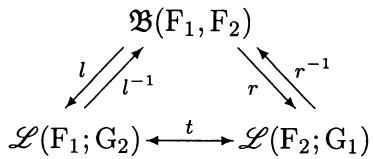
\includegraphics[keepaspectratio]{images/part003_fb3d81cd.jpg}}

where t is the isomorphism of transposition \(u \mapsto {}^{t}u\) . In view of the definition of the weak topologies on \(G_{1}\) and \(G_{2}\) , it is moreover immediate that when \(\mathfrak{B}(F_{1}, F_{2})\) , \(\mathcal{L}(F_{1}; G_{2})\) and \(\mathcal{L}(F_{2}; G_{1})\) are equipped with the topology of pointwise convergence, the isomorphisms in the preceding diagram are isomorphisms for the topological vector space structures.

Now let E, F be two Hausdorff locally convex spaces, \(E'\) , \(F'\) their respective duals; we denote by \(E_{\sigma}\) , \(F_{\sigma}\) the spaces E, F equipped with the weakened topologies \(\sigma(\mathrm{E}, \mathrm{E}')\) , \(\sigma(\mathrm{F}, \mathrm{F}')\) , and by \(E_{s}'\) , \(F_{s}'\) the spaces \(E'\) , \(F'\) equipped with the weak topologies \(\sigma(\mathrm{E}', \mathrm{E})\) , \(\sigma(\mathrm{F}', \mathrm{F})\) . Thus, the preceding remarks establish canonical isomorphisms between the three spaces \(\mathfrak{B}(\mathrm{E}_{\sigma}, \mathrm{F}_{s}')\) , \(\mathcal{L}(\mathrm{E}_{\sigma}; \mathrm{F}_{\sigma})\) and \(\mathcal{L}(\mathrm{F}_{s}'; \mathrm{E}_{s}')\) , and also between the three spaces \(\mathfrak{B}(\mathrm{E}_{\sigma}, \mathrm{F}_{\sigma})\) , \(\mathcal{L}(\mathrm{E}_{\sigma}; \mathrm{F}_{s}')\) and \(\mathcal{L}(\mathrm{F}_{\sigma}; \mathrm{E}_{s}')\) . One will observe that \(\mathfrak{B}(\mathrm{E}_{\sigma}, \mathrm{F}_{\sigma})\) is also equal to the space \(\mathfrak{B}(\mathrm{E}, \mathrm{F})\) of separately continuous bilinear forms on \(E \times F\) (E and F being equipped with their original topologies), since every continuous linear form on E (resp. F) is continuous on \(E_{\sigma}\) (resp. \(F_{\sigma}\) ) and conversely (TVS, II, §6, No.~1 and No.~2, Prop. 3).

Let \(\mathcal{B}(\mathrm{E},\mathrm{F})\) be the space of continuous bilinear forms on \(\mathbf{E}\times \mathbf{F}\) (E and F being equipped with their original topologies); then \(\mathcal{B}(\mathrm{E},\mathrm{F})\subset \mathfrak{B}(\mathrm{E},\mathrm{F})\) .

PROPOSITION 1. --- For a bilinear form \(\Phi \in \mathfrak{B}(\mathrm{E},\mathrm{F})\) to belong to \(\mathcal{B}(\mathrm{E},\mathrm{F})\) , it is necessary and sufficient that there exist a neighborhood of 0 in E whose image under \(^l\Phi\) is an equicontinuous subset of \(\mathbf{F}'\) .

For, to say that \(\Phi\) is continuous means that there exists a balanced convex neighborhood V (resp. W) of 0 in E (resp. F) such that \(|\Phi(x,y)| \leqslant 1\) for \(x \in V\) , \(y \in W\) ; this may be written \(|\langle^{l}\Phi(x), y \rangle| \leqslant 1\) for \(x \in V\) , \(y \in W\) , or also \(^{l}\Phi(V) \subset W^{\circ}\) ; whence the proposition, taking into account the fact that every equicontinuous subset of \(F'\) is contained in the polar of a neighborhood of 0 in F.

COROLLARY. --- If \(\Phi\) is a continuous bilinear form on \(\mathbf{E} \times \mathbf{F}\) , then \(^l\Phi\) is a continuous linear mapping of \(\mathbf{E}\) into the strong dual \(\mathbf{F}_b'\) of \(\mathbf{F}\) . If, moreover, \(\mathbf{E}\) and \(\mathbf{F}\) are normed spaces, then \(\|^l\Phi\| = \| \Phi \|\) .

The first assertion follows from Prop. 1 and the fact that every neighborhood of 0 in \(F_{b}^{\prime}\) absorbs every equicontinuous subset of \(F^{\prime}\) . If E and F are normed, then

\[
\begin{array}{c} \| \Phi \| = \sup _ {\| x \| \leqslant 1, \| y \| \leqslant 1} | \Phi (x, y) | = \sup _ {\| x \| \leqslant 1} \Big (\sup _ {\| y \| \leqslant 1} \big | \langle^ {l} \Phi (x), y \rangle \big | \Big) \\ = \sup _ {\| x \| \leqslant 1} \| ^ {l} \Phi (x) \| = \| ^ {l} \Phi \|, \end{array}
\]

whence the second assertion.

Interchanging the roles of E and F, one obtains results analogous to Prop. 1 and its corollary for the linear mappings \(r\Phi\) ; we leave to the reader the task of stating them.

\section{Some types of spaces having the property (GDF)}

We already know that every Fréchet space has the property (GDF) (TVS, I, §3, No.~3, Cor. 5 of Th. 1).

PROPOSITION 2. --- Let E be a vector space, \((\mathrm{F}_{\alpha})_{\alpha\in\mathrm{A}}\) a family of locally compact spaces having the property (GDF), and for each \(\alpha\in A\) let \(h_{\alpha}\) be a linear mapping of \(F_{\alpha}\) into E. If E is equipped with the finest locally convex topology that makes the \(h_{\alpha}\) continuous, then E has the property (GDF).

Let \(u\) be a linear mapping of \(\mathbf{E}\) into a Banach space \(\mathbf{B}\) , such that every limit in \(\mathbf{E} \times \mathbf{B}\) of every convergent sequence of points of the graph \(\Gamma\) of \(u\) also belongs to \(\Gamma\) . It suffices to show that, for every \(\alpha \in \mathbf{A}\) , \(u \circ h_{\alpha}\) is continuous on \(\mathrm{F}_{\alpha}\) (TVS, II, §4, No.~4, Prop. 5). Now, let \((x_n)\) be a sequence of elements of \(\mathrm{F}_{\alpha}\) having a limit \(a\) and such that the sequence \(\left(u(h_{\alpha}(x_n))\right)\) has a limit \(b \in \mathbf{B}\) . Since \(h_{\alpha}\) is continuous, \(h_{\alpha}(a)\) is a limit of the sequence \((h_{\alpha}(x_n))\) in \(\mathbf{E}\) ; therefore by hypothesis \(b = u(h_{\alpha}(a))\) and, since \(\mathrm{F}_{\alpha}\) has the property (GDF), \(u \circ h_{\alpha}\) is continuous.

COROLLARY. --- Every quotient space of a locally convex space having the property (GDF) has the property (GDF).

PROPOSITION 3. --- The strong dual of a reflexive Fréchet space has the property (GDF).

This is a consequence of Prop. 2 and the following lemma (or TVS, IV, §3, No.~4, Prop. 4):

Lemma. --- Let F be a Fréchet space, \(F'\) its strong dual, \(F''\) its bidual. If every subset of \(F''\) , bounded for \(\sigma(F'', F')\) , is contained in the closure (for \(\sigma(F'', F')\) ) of a bounded subset of F, then \(F'\) is the direct limit of a sequence of Banach spaces.

For, let \((\mathrm{V}_{n})\) be a decreasing fundamental sequence of convex, balanced and closed neighborhoods of 0 in F. For every integer n, let \(G_{n}\) be the linear subspace of \(F'\) generated by the polar \(V_{n}^{\circ}\) of \(V_{n}\) . In \(G_{n}\) , \(V_{n}^{\circ}\) is an absorbent convex set, therefore its gauge \(p_{n}\) is a norm on \(G_{n}\) ; moreover, \(V_{n}^{\circ}\) is a complete subset of the strong dual \(F'\) (TVS, III, §3, No.~8, Prop. 11); thus \(G_{n}\) , equipped with the norm \(p_{n}\) , is a Banach space (GT, III, §3, No.~5, Cor. 2 of Prop. 9). We are going to show that the strong topology on \(F'\) is the direct limit of these Banach space topologies on the \(G_{n}\) , or again that, for a strongly closed, balanced, convex subset U of \(F'\) to be a strong neighborhood of 0, it is necessary and sufficient that it absorb each of the \(V_{n}^{\circ}\) . It is obvious that this condition is necessary; to see that it is sufficient, it will suffice to prove that U contains a barrel of \(F'\) . Indeed, its polar \(U^{\circ}\) in \(F''\) will then be bounded for \(\sigma(\mathrm{F}''\mathrm{,}\mathrm{F}')\) , hence, by hypothesis, will be contained in the closure (for \(\sigma(\mathrm{F}''\mathrm{,}\mathrm{F}')\) ) of a bounded subset B of F, from which one can conclude that U (which is closed for \(\sigma(\mathrm{F}^{\prime},\mathrm{F}''\mathrm{)})\) ) contains the strong neighborhood \(B^{\circ}\) of 0 (TVS, II, §6, No.~3, Th. 1 and §8, No.~4).

By hypothesis, for every integer n there exists a number \(\lambda_{n}>0\) such that \(\lambda_{n}V_{n}^{\circ}\subset\frac{1}{2}U\) ; let \(A_{n}\) be the convex envelope of the union of the \(\lambda_{i}V_{i}^{\circ}\) for \(i\leqslant n\) . Then \(A_{n}\subset\frac{1}{2}U\) for every n; let W be the union of the \(A_{n}\) ; W is a convex, balanced, absorbent set contained in \(\frac{1}{2}U\) , and it will suffice to show that its strong closure (which is a barrel) is contained in U.

Thus, let \(x'\) be a point of \(F'\) not belonging to U. Since each of the \(V_n^\circ\) is compact for \(\sigma(F', F)\) , the same is true of the \(A_n\) (TVS, II, §2, No.~6, Prop. 15), and since \(x' \notin 2A_n\) , there exists an element \(x_n\) belonging to the polar of \(A_n\) in F such that \(\langle x', x_n \rangle = 2\) (TVS, II, §5, No.~3, Prop. 4). The sequence \((x_n)\) is bounded in F: for, every \(y' \in F'\) belongs to some \(V_k^\circ\) , consequently \(|\langle y', x_n \rangle| \leqslant \lambda_k^{-1}\) for \(n \geqslant k\) , whence our assertion (TVS, IV, §1, No.~1, Prop. 1). Let C be a bounded, balanced convex set in F containing all the \(x_n\) ; \(C^\circ\) is then a neighborhood of 0 in \(F'\) , and the polar \(C^{\circ\circ}\) of \(C^\circ\) in \(F''\) is compact for \(\sigma(F'', F')\) (TVS, III, §3, No.~4, Cor. 2 of Prop. 4 and No.~5, Prop. 7). Thus one sees that the sequence \((x_n)\) has a cluster point \(x''\) in \(F''\) for \(\sigma(F'', F')\) ; obviously \(\langle x', x'' \rangle = 2\) and, on the other hand, \(x''\) belongs to the polar of \(A_n\) in \(F''\) for every \(n\) , hence to the polar \(W^\circ\) of W in \(F''\) . From this, one concludes that \(x' \notin W^{\circ\circ}\) , hence is not in the closure of W for \(\sigma(F', F'')\) (TVS, II, §6, No.~3, Th. 1 and §8, No.~4), therefore a fortiori for the strong topology, which completes the proof.
